\documentclass[11pt]{article}
\usepackage[margin=1in]{geometry}
\usepackage{amsmath, amssymb}
\usepackage{graphicx}
\usepackage{booktabs}
\usepackage{xcolor}

\definecolor{garnet}{HTML}{73000A}
\definecolor{black90}{HTML}{363636}

\color{black90}

\title{\color{garnet}\textbf{Exercise 5.1 --- Blackjack Value Function Analysis}}
\author{J.C.\ Vaught}
\date{Spring 2026 --- CSCE 775}

\begin{document}
\maketitle

\section*{Problem Statement}

Consider the diagrams on the right in Figure~5.1 (the 500{,}000-episode surfaces). The exercise poses three questions.

\begin{enumerate}
    \item Why does the estimated value function jump up for the last two rows in the rear?
    \item Why does it drop off for the whole last row on the left?
    \item Why are the frontmost values higher in the upper diagrams (usable ace) than in the lower (no usable ace)?
\end{enumerate}

\section*{Setup Recap}

The policy evaluated is simple: \textit{stick} if the player's current sum is 20 or 21, and \textit{hit} otherwise. The state is a triple $(s_{\text{player}},\; d_{\text{showing}},\; \text{usable ace})$ where $s_{\text{player}} \in \{12, 13, \ldots, 21\}$ and $d_{\text{showing}} \in \{A, 2, \ldots, 10\}$. Rewards are $+1$ (win), $0$ (draw), $-1$ (loss), with $\gamma = 1$.

\section*{Reproduced Figure}

The following figure was generated by running first-visit Monte Carlo prediction with 10{,}000 and 500{,}000 episodes using the stick-on-20-or-21 policy.

\begin{figure}[h]
    \centering
    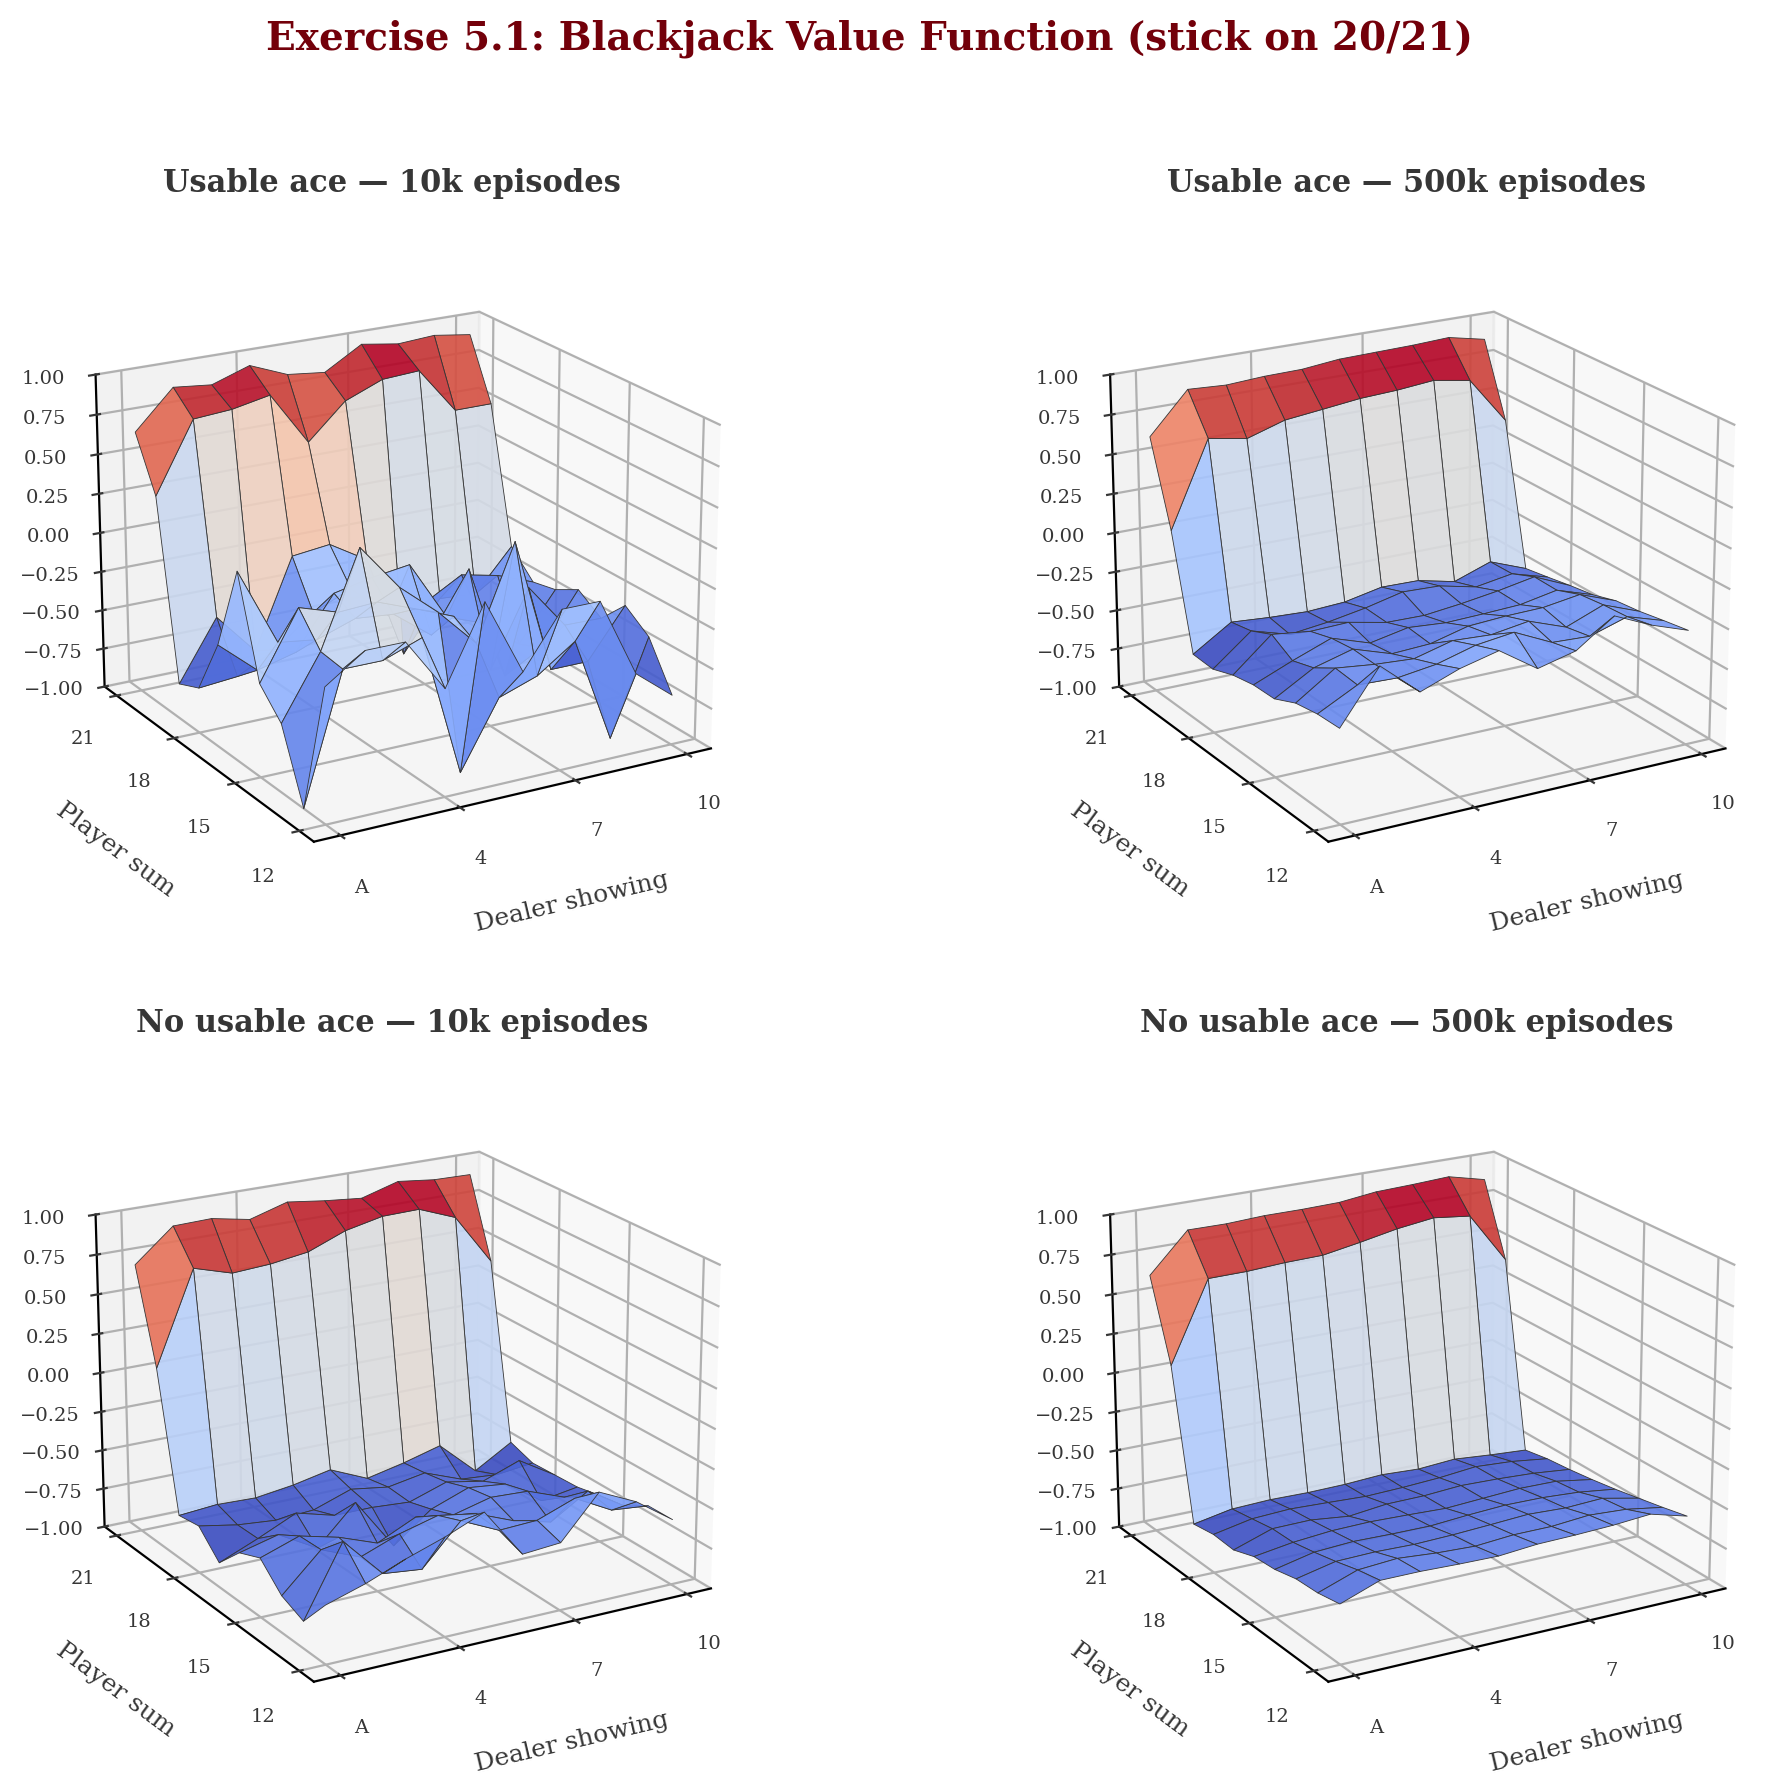
\includegraphics[width=0.85\textwidth]{blackjack_value_function.png}
    \caption{Approximate state-value functions for the blackjack stick-on-20-or-21 policy, computed via first-visit MC evaluation.}
\end{figure}

\section*{Answer 1: Why does the value function jump up for the last two rows in the rear?}

The ``last two rows in the rear'' correspond to player sums of \textbf{20 and 21}. Under the evaluated policy, the player \textit{sticks} at these sums. A player holding 20 or 21 is in an extremely strong position because the dealer must beat that total without busting.

The value jumps sharply because of a qualitative change in the policy's behavior at these states. For player sums 12--19 the player keeps hitting and risks busting, producing predominantly negative expected returns. At sum 20 the player sticks, and the dealer must draw 21 to win (or exactly 20 to tie). At sum 21 the situation is even more favorable. Numerically, from the 500{,}000-episode simulation:

\begin{table}[h]
    \centering
    \begin{tabular}{ccc}
        \toprule
        Player Sum & $V$ (vs.\ Dealer Ace) & $V$ (vs.\ Dealer 10) \\
        \midrule
        19 & $-0.779$ & $-0.746$ \\
        20 & $+0.148$ & $+0.436$ \\
        21 & $+0.640$ & $+0.888$ \\
        \bottomrule
    \end{tabular}
    \caption{Sharp jump at the policy's stick threshold (no usable ace case).}
\end{table}

The jump from 19 to 20 is nearly a full unit of reward. This discontinuity arises precisely because the policy switches from \textit{hit} (high bust risk with sums like 19) to \textit{stick} (strong final hand). In fact, hitting on 19 is a terrible decision---there is only a $1/13$ chance of drawing an ace (to reach 20) and a $2/13$ chance of reaching 21, but a $10/13$ probability of busting---which is why the policy performs poorly for sums just below 20.

\section*{Answer 2: Why does the value function drop off for the whole last row on the left?}

The ``last row on the left'' corresponds to the dealer showing an \textbf{ace} (card value 1). The dealer's ace is the strongest possible up-card for two reasons.

First, the ace gives the dealer a \textit{usable ace}, meaning the dealer's hand is flexible. The dealer can count the ace as 11 when beneficial and revert to 1 if the subsequent total exceeds 21. This flexibility significantly reduces the dealer's probability of busting.

Second, the dealer has a high probability of reaching strong totals (17--21) when starting with an ace. The probability that the dealer busts given a showing ace is only about 11.5\%, compared with roughly 40\% when showing a 5 or 6. Since the dealer busts less often, the player wins less often, and the value function is lower across all player sums when the dealer shows an ace.

This effect is visible across the entire surface: for every player sum from 12 to 21, the value is lowest when the dealer shows an ace compared to any other up-card.

\section*{Answer 3: Why are the frontmost values higher with a usable ace than without?}

The ``frontmost values'' correspond to \textbf{low player sums} (12, 13, 14, \ldots). In these states the player is hitting under the policy. Having a usable ace provides a crucial safety net.

When the player holds a usable ace, any hit that would cause a bust can be absorbed by converting the ace from 11 to 1. For example, a player with sum 15 and a usable ace (really holding an ace counted as 11 plus a 4) who draws a 9 would reach $15 + 9 = 24$. But the ace converts to 1, bringing the total to $14$, and the player continues without busting.

Without a usable ace, the same draw causes an immediate bust and a $-1$ reward. This makes the expected return for low player sums significantly worse in the no-usable-ace case, because the player is forced to hit (the policy says hit below 20) and every hit carries real bust risk.

Quantitatively, comparing the two cases at player sum 12 against a dealer 10:
\begin{align}
    V(\text{usable ace, sum 12, dealer 10}) &= -0.279 \\
    V(\text{no usable ace, sum 12, dealer 10}) &= -0.567
\end{align}
The usable-ace state is nearly twice as favorable because the player can absorb bad draws. As the player sum increases toward 20, this advantage shrinks because even with a usable ace, high sums leave little room for improvement. At sums 20 and 21 the player sticks regardless, so the usable-ace distinction barely matters for those terminal policy states.

\section*{Summary}

\begin{table}[h]
    \centering
    \begin{tabular}{p{0.22\textwidth} p{0.68\textwidth}}
        \toprule
        \textbf{Feature} & \textbf{Explanation} \\
        \midrule
        Jump at sums 20--21 & The policy switches from hit to stick. Sticking on 20 or 21 produces strong outcomes; hitting on 19 or below risks busting. \\
        \addlinespace
        Drop at dealer ace & The dealer's ace is the strongest up-card: it minimizes dealer bust probability through flexible ace counting, reducing the player's expected reward. \\
        \addlinespace
        Higher front values with usable ace & A usable ace prevents busting on hits by converting 11 to 1, acting as insurance during the forced-hitting phase (sums 12--19). \\
        \bottomrule
    \end{tabular}
\end{table}

\end{document}
